%!TEX root = ../A_Novel_Filtering_Approach_for_Robust_and_Fast_Keypoint_Matching_in_Mobile_Environment.tex

\subsection{Proof of Criteria}
\subsubsection{Validation Design}
% 제안하는 keypoint evaluation criteria 를 검증하기 위하여, 우리는 각 keypoint 들의 correct matching count 를 기준으로 제안된 criteria의 연관성을 측정하였다. 먼저, 우리는 robust image matching 환경을 고려하여, 다양한 변환을 적용한 dataset을 생성하였다. 그리고 이러한 dataset을 기반으로, 각 keypoint 별로 correct matching count 를 측정하여 matching quality 에 대한 ground truth data를 계산하였다.
To validate the proposed keypoint evaluation criteria, we examined a relationship between criteria and correct matching count of each keypoints. At first, to provide robust image matching, we synthesized image dataset by various image transformation. Then, based on this dataset, we counted correct matching count for each keypoint, and this correct matching count is a basis of matching quality. 이러한 correct matching count가 높은 특징점은 fixed image dataset 에서 더 높은 matching quality를 보여준다고 볼 수 있기 때문에 본 논문에서 제안하는 Matching에 더 적합한 keypoint로 볼 수 있다. 반대로 correct matching count가 낮은 특징점은 특징점이 반복적으로 검출되지 않거나, 모호성이 높아 inter-keypoint miss-match가 많이 발생하는 특징점으로 matching에 적합하지 못한 keypoint로 볼 수 있다. 따라서, 이러한 correct match count 와 제안하는 keypoint evaluation score function (see, Eq. \ref{eq:score_function}) 간의 상관관계를 관찰함으로써 제안하는 score function 의 적절성을 검증할 수 있다.

% Genuine / Impostor 분포에 관한 얘기

\subsubsection{Dataset}
검증에 사용된 이미지는 서울 관광 가이드북\cite{_seoul_2014}의 \textit{Seoul Tour Map} 16장을 사용하였다. 우리는 이러한 이미지를 대상으로 rotate($0.5-2.0$-folds, at the interval of 0.1-fold), scaling($0\degree-360\degree$, at the interval of $10$ intervals), and blurring (Gaussian blur, $r \in \left \{ 0, 3, 5, 7 \right \}$ pixels) 의 transform을 적용하여 총 36,864 장의 dataset을 생성하였다. 이 중 랜덤으로 training Set 16,114 장, Test set 16,142 장을 선택하여 실험을 진행하였다. 

\subsubsection{Images Patches}
그림 \ref{fig:image_patches}와 같이, correct matching count 를 기준으로 상위 10개의 keypoint 와 하위 10개의 keypoint 들의 특징을 비교하였다. 상위 10개에 대한 패치는 비교적 단순한 사각형 형태에서 많이 검출되었다. Genuine과 Impostor Histogram의 값을 정규화하여 표현된 Normal Distribution의 분포를 보면 Genuine과 Impostor 분포가 확연하게 구분되는 것을 확인할 수 있다. 반면, 하위 10개에 대한 패치는 글자 또는 단순한 패턴이 반복되는 형태에서 많이 검출되었다. Genuine과 Impostor Histogram의 값을 정규화하여 표현된 Normal Distribution의 분포를 보면 Genuine과 Impostor 분포가 많은 부분 겹쳐있어 구분이 어려운 것을 확인할 수 있다. 
인식에 좋은 특징점은 큰 숫자 패치와 같이 단순한 색상으로 패턴이 큰 숫자 표지와 같은 특징점이 인식에 좋은 성능을 보여주었으며, 반대로 작은 설명 글씨와 같은 특징점들은 인식 성능이 좋지 못하였으며, 이러한 점들을 제거하고 학습을 수행하는 것이 좋다.


\begin{figure}[htb!]
  \centering     %%% not \center
    \subfloat[the best 100-images]{\label{fig:patches_good}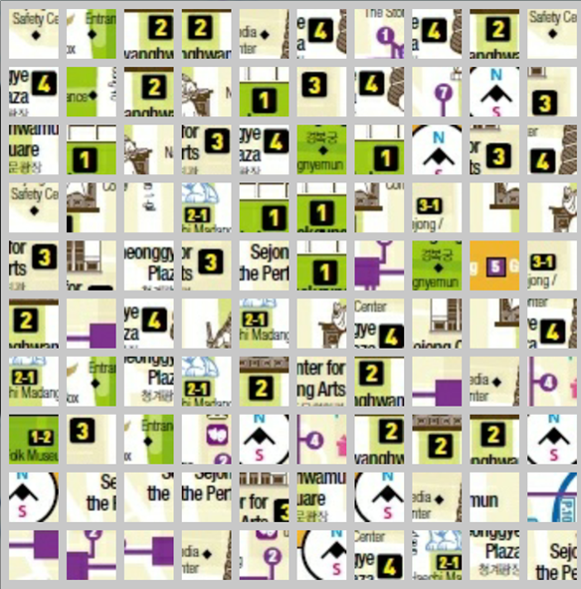
\includegraphics[width=0.45\textwidth]{3_proposed/patch_good}}
    % 
\\
    \subfloat[the worst 100-images]{\label{fig:patches_bad}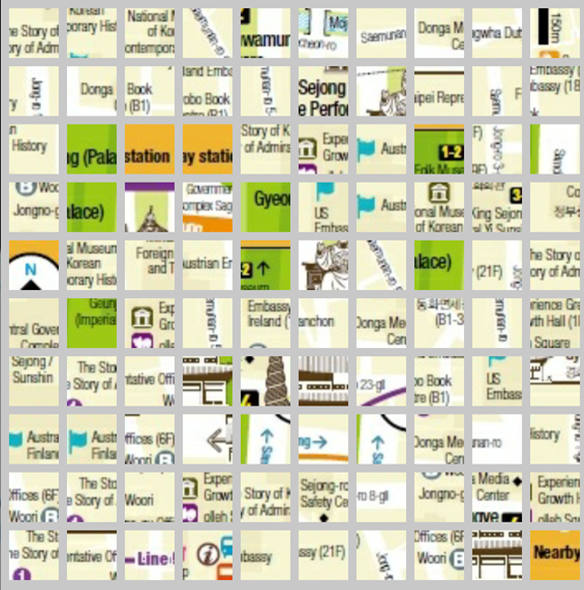
\includegraphics[width=0.45\textwidth]{3_proposed/patch_bad}}
  \caption{The Best/Worst 100-Images with Regard to Correct Matching Count}
    \label{fig:image_patches}
\end{figure}

